\documentclass{class}

\usepackage[table]{xcolor}% http://ctan.org/pkg/xcolor
\usetikzlibrary{positioning}
\usepackage{adjustbox}
\usepackage{bbm}
\usepackage{mathrsfs}  
\usepackage{amsmath}% http://ctan.org/pkg/amsmath
\usepackage{tcolorbox}
\setbeamerfont{itemize/enumerate subbody}{size=\normalfont}
\setbeamerfont{itemize/enumerate subsubbody}{size=\normalfont}
\setbeamertemplate{itemize item}{$\bullet$}
\setlength{\leftmargini}{0.25cm}

\title{Self-Selection in Retail Electricity Contracts}
\subtitle{Competition, Regulation, and Welfare Implications}

\author{Léopold Monjoie, Julien Duc}
\institute{Aalto University \and Université Paris Dauphine, PSL Research University, LEDa}


\apptocmd{\frame}{}{\justifying}{}
\newcommand{\sign}{\text{sign}}
% Conference on Economic Design

\bibliographystyle{apalike}

\begin{document}

\newlength{\tempb}

\frame{\titlepage}

\newcommand{\commentedbox}[2]{%
  \mbox{
    \begin{tabular}[t]{@{}c@{}}
    $\boxed{\displaystyle#1}$\\
    #2
    \end{tabular}%
  }%
}

\newcommand\Wider[2][3em]{%
\makebox[\linewidth][c]{%
  \begin{minipage}{\dimexpr\textwidth+#1\relax}
  \raggedright#2
  \end{minipage}%
  }%
}

\newcommand*\circled[1]{\tikz[baseline=(char.base)]{
            \node[shape=circle,draw,inner sep=2pt] (char) {#1};}}

%%%%%%%%%%%%%%%%%%%%%%%%%%%%%%%%%%%%%%%%%%%%%%%%%%%%%%%%%%%%%%%%%%%%%%%%%%%%%%%%%%%%%%%%%%%%%%%%%%%%%%%%%%%%%%%%%%%%%%%%%%%%%%%%%%%%%%%%%%%%%%%%%%%%%%


\section{Introduction and motivations}


\begin{frame}{Motivations}\label{Motivations}

\begin{mainbox}{Question}
How do consumers self-select into contracts in retail electricity markets?
\end{mainbox}

\vfill

\begin{itemize}
    \item Contracts define how wholesale prices are transmitted to final consumers. \vfill
\begin{itemize}
    \item First-best: when every consumer is fully exposed to prices from a perfectly competitive wholesale market (RTP). \vfill
    \item Different contract choices $\rightarrow$ inefficiencies.\vfill
    \item \hyperlink{Lit_FB}{\beamergotobutton{Literature}} \vfill
\end{itemize}

\end{itemize}

\begin{mainbox}{This paper}
We study under which environment letting consumers choose their contract can lead to adverse selection. (\textit{private vs. public firms})
\end{mainbox}
       
\end{frame}

% %%%%%%%%%%%%%%%%%%%%%%%%%%%%%%%%%%%%%%%%%%%%%%%%%%%%%%%%%%%%%%%%%%%%%%%%%%%%%%%%%%%%%%%%%%%%%%%%%%%%%%%%%%%%%%%%%%%%%%%%%%%%%%%%%%%%%%%%%%%%%%%%%%%%%%


\begin{frame}{Dynamic contracts uptake remains low }\label{UptakeContract1}

\begin{figure}
    \centering
    
\includegraphics[width=1\linewidth]{figure/FP_EU.PNG}
    \caption{Fixed-price contracts as a share of household contracts in Europe \cite{ACER2024} \hyperlink{options1}{\beamergotobutton{Options}}} 
    \label{fig:FP_EU}
\end{figure}

\end{frame}

%%%%%%%%%%%%%%%%%%%%%%%%%%%%%%%%%%%%%%%%%%%%%%%%%%%%%%%%%%%%%%%%%%%%%%%%%%%%%%%%%%%%%%%%%%%%%%%%%%%%%%%%%%%%%%%%%%%%%%%%%%%%%%%%%%%%%%%%%%%%%%%%%%%%%%

\begin{frame}{First contribution: Demand for contracts with heterogeneous consumers}\label{FirstCont}


\begin{itemize}

\item \textbf{Who selects which type of contracts?} \vfill

\item Provide a \boldrblue{stylized theoretical framework} where a set of consumers have to choose between \boldrblue{a Fixed-Price contract} or \boldrblue{a RTP contract}. 

\vfill

\item Consumers can consume over \boldrblue{two periods} with \boldrblue{different willingness-to-pay} in each period. 

\vfill

\item Assume entirely rational and risk-neutral consumers.

\vfill

\end{itemize}

\begin{mainbox}{Contribution}
Provide \boldrblue{the demand} for each contract, given a set of prices and the type of consumers who choose each contract.  
\end{mainbox}

\vfill

\begin{itemize}

\item Literature \hyperlink{Lit_Conso}{\beamergotobutton{Contracts and Electricity Markets}} 
\end{itemize}



\end{frame}

% %%%%%%%%%%%%%%%%%%%%%%%%%%%%%%%%%%%%%%%%%%%%%%%%%%%%%%%%%%%%%%%%%%%%%%%%%%%%%%%%%%%%%%%%%%%%%%%%%%%%%%%%%%%%%%%%%%%%%%%%%%%%%%%%%%%%%%%%%%%%%%%%%%%%%%

\begin{frame}{Private contracts coexist with regulated options }\label{UptakeContract2}

\begin{figure}
    \centering
    
\includegraphics[width=1\linewidth]{figure/FP_EU_detail.PNG}
    \caption{Share of household contract uptake in Europe \cite{ACER2024} \hyperlink{options1}{\beamergotobutton{Options}}} 
    \label{fig:FP_EU_detail}
\end{figure}

\end{frame}

%%%%%%%%%%%%%%%%%%%%%%%%%%%%%%%%%%%%%%%%%%%%%%%%%%%%%%%%%%%%%%%%%%%%%%%%%%%%%%%%%%%%%%%%%%%%%%%%%%%%%%%%%%%%%%%%%%%%%%%%%%%%%%%%%%%%%%%%%%%%%%%%%%%%%%

\begin{frame}{Second contribution: Market consequences of consumer choices}\label{SecondCont}


\begin{itemize}

\item \textbf{Does the market structure matter with contract self-selection}?  

\vfill

\item We model \boldrblue{retail competition} between firms that offer the two contracts. 

\vfill

\item Two \boldrblue{market structures} depending on the type of firms.

\begin{itemize}
    \item Perfectly competitive retailers always offer the RTP contract.
    \item Either the same retailers or a regulated monopoly offer the FP contract.
\end{itemize}

\end{itemize}


\vfill

\begin{mainbox}{Contribution}
We characterize \boldrblue{the price and welfare equilibrium} in the retail market in each market structure when consumers can self-select into the offered contracts.
\end{mainbox}

\vfill

\begin{itemize}
\item Literature \hyperlink{Lit_Mkt1}{\beamergotobutton{Retail Competition in Electricity Markets}}  and \hyperlink{Lit_Mkt2}{\beamergotobutton{General Theory}} 
\end{itemize}


\end{frame}

%%%%%%%%%%%%%%%%%%%%%%%%%%%%%%%%%%%%%%%%%%%%%%%%%%%%%%%%%%%%%%%%%%%%%%%%%%%%%%%%%%%%%%%%%%%%%%%%%%%%%%%%%%%%%%%%%%%%%%%%%%%%%%%%%%%%%%%%%%%%%%%%%%%%%%

\begin{frame}{Main takeaways}


\begin{itemize}

\item \boldrblue{Demand for contracts}.

\vfill

\begin{itemize} 
    \item Higher w.t.p. during \boldrblue{low-price} periods $\rightarrow$ RTP contract.\vfill
    \item Higher w.t.p. during \boldrblue{high-price} periods $\rightarrow$ FP contract.\vfill
    \item Key ingredient: the indifferent consumer. 
\end{itemize}

\vfill

\item \boldrblue{Market Equilibrium}.

\vfill

\begin{itemize}
    \item When there are only competitive retailers on the market, only the RTP contract is offered $\rightarrow$ \boldrblue{No Adverse Selection}. \vfill

    \begin{itemize}
        \item \textit{Competition excludes costly consumers.} \vfill
    \end{itemize}
    \item When the regulated firm offers the FP contract, there exists a demand for the FP contract $\rightarrow$ \boldrblue{Adverse Selection} \vfill

    \begin{itemize}
        \item \textit{Leakage between the public/private firms lead to low inefficient prices.} 
    \end{itemize}
\end{itemize}



\end{itemize}


\end{frame}

%%%%%%%%%%%%%%%%%%%%%%%%%%%%%%%%%%%%%%%%%%%%%%%%%%%%%%%%%%%%%%%%%%%%%%%%%%%%%%%%%%%%%%%%%%%%%%%%%%%%%%%%%%%%%%%%%%%%%%%%%%%%%%%%%%%%%%%%%%%%%%%%%%%%%%
% %%%%%%%%%%%%%%%%%%%%%%%%%%%%%%%%%%%%%%%%%%%%%%%%%%%%%%%%%%%%%%%%%%%%%%%%%%%%%%%%%%%%%%%%%%%%%%%%%%%%%%%%%%%%%%%%%%%%%%%%%%%%%%%%%%%%%%%%%%%%%%%%%%%%%%
% %%%%%%%%%%%%%%%%%%%%%%%%%%%%%%%%%%%%%%%%%%%%%%%%%%%%%%%%%%%%%%%%%%%%%%%%%%%%%%%%%%%%%%%%%%%%%%%%%%%%%%%%%%%%%%%%%%%%%%%%%%%%%%%%%%%%%%%%%%%%%%%%%%%%%%

\section{The model}

% \subsection{The environment}

\begin{frame}{Roadmap}
  \tableofcontents [sectionstyle=show/shaded,subsectionstyle=show/shaded]
\end{frame}


%%%%%%%%%%%%%%%%%%%%%%%%%%%%%%%%%%%%%%%%%%%%%%%%%%%%%%%%%%%%%%%%%%%%%%%%%%%%%%%%%%%%%%%%%%%%%%%%%%%%%%%%%%%%%%%%%%%%%%%%%%%%%%%%%%%%%%%%%%%%%%%%%%%%%%


\begin{frame}{Timing}


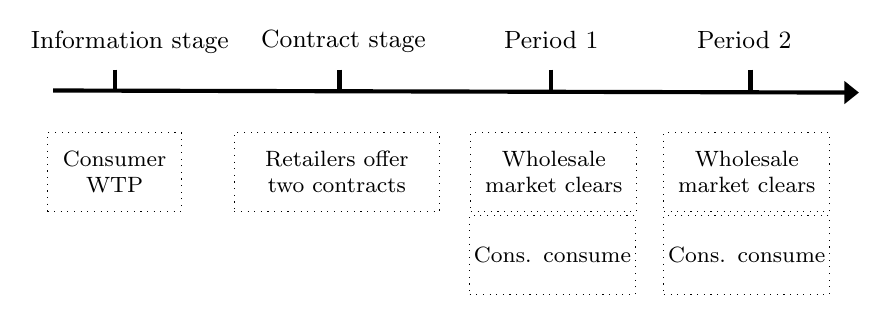
\begin{tikzpicture}[x=0.45pt,y=0.75pt,yscale=-1,xscale=1]

\draw [line width=1.5]    (20,100) -- (663,101) ;
\draw [shift={(667,101)}, rotate = 180.07] [fill={rgb, 255:red, 0; green, 0; blue, 0 }  ][line width=0.08]  [draw opacity=0] (11.61,-5.58) -- (0,0) -- (11.61,5.58) -- cycle    ;
\draw [line width=1.5,color = black]    (70,90) -- (70,100) ;
\draw [line width=1.5,color = black]   (250,90) -- (250,100) ;
\draw [line width=1.5,color = black]   (420,90) -- (420,100)  ;
\draw [line width=1.5,color = black]    (580,90) -- (580,100)   ;

% Text Node
\draw (0,70) node [anchor=north west][inner sep=0.75pt]  [font=\small] [align=center] {Information stage};
\draw (185,70) node [anchor=north west][inner sep=0.75pt]  [font=\small] [align=center] {Contract  stage};
\draw (380,70) node [anchor=north west][inner sep=0.75pt]  [font=\small] [align=center] {Period 1};
\draw (535,70) node [anchor=north west][inner sep=0.75pt]  [font=\small] [align=center] {Period 2};

\draw (15,120) node [draw = black,anchor=north west,minimum height = 1 cm,  text  width = 1.6cm][inner sep=1.5pt,dotted]  [font=\footnotesize] [align=center] {Consumer WTP};
% \draw (15,160) node [anchor=north west,minimum height = 1 cm,  text  width = 1.6cm,dotted][inner sep=1.5pt]  [font=\footnotesize] [align=center] { \textit{common info.} \\ \textit{private info.}};

\draw (165,120) node [draw = black,anchor=north west,minimum height = 1 cm,  text  width = 2.5cm][inner sep=1.5pt,dotted]  [font=\footnotesize] [align=center]{ Retailers offer \\ two contracts};
\draw (355,120) node [draw = black,anchor=north west,minimum height = 1 cm,  text  width =  2cm,dotted][inner sep=1.5pt]  [font=\footnotesize] [align=center] { Wholesale  \\ market clears};
\draw (354,160) node [draw = black,anchor=north west,minimum height = 1 cm,  text  width = 2cm,dotted][inner sep=1.5pt]  [font=\footnotesize] [align=center] { Cons. consume};

\draw (510,120) node [draw = black,anchor=north west,minimum height = 1 cm,  text  width = 2cm,dotted][inner sep=1.5pt]  [font=\footnotesize] [align=center] { Wholesale  \\ market clears};
\draw (510,160) node [draw = black,anchor=north west,minimum height = 1 cm,  text  width = 2cm,dotted][inner sep=1.5pt]  [font=\footnotesize] [align=center] { Cons. consume};

\end{tikzpicture}

    
\end{frame}


% %%%%%%%%%%%%%%%%%%%%%%%%%%%%%%%%%%%%%%%%%%%%%%%%%%%%%%%%%%%%%%%%%%%%%%%%%%%%%%%%%%%%%%%%%%%%%%%%%%%%%%%%%%%%%%%%%%%%%%%%%%%%%%%%%%%%%%%%%%%%%%%%%%%%%%

\begin{frame}{Consumers and retailers}

\begin{itemize}
    \item A unit mass of consumers with a \boldrblue{unit demand} for each $t = 1,2$. 

\vfill

    \item W.t.p: a \boldrblue{two-dimensional} type $\textbf{v}=(v_1,v_2) $. Drawn from a uniform pdf. $f_t(v)$ and cdf. $F_t(v)$ with support $[\underline{v}_t,\bar{v}_t]$.  

        \vfill
        
\begin{equation*}
U^k\left(\textbf{v},\textbf{p}\right)= v_1-p^k_1 +  v_2-p^k_2
\end{equation*}    

     \vfill

\item We assume a set of retailers that purchase at \boldrblue{no additional cost} on the wholesale market.  \vfill

\item If $\textbf{p}^k=(p_1^k,p_2^k)$ is profile price of contract $k$, then:  \vfill

    \begin{itemize}
        \item FP contract: $\textbf{p}^{r} =  (p_r,p_r)$ \vfill
        \item RTP contract: $\textbf{p}^{s} =  (p_1,p_2)$
    \end{itemize}
    
\end{itemize}    
\end{frame}

% %%%%%%%%%%%%%%%%%%%%%%%%%%%%%%%%%%%%%%%%%%%%%%%%%%%%%%%%%%%%%%%%%%%%%%%%%%%%%%%%%%%%%%%%%%%%%%%%%%%%%%%%%%%%%%%%%%%%%%%%%%%%%%%%%%%%%%%%%%%%%%%%%%%%%%

\begin{frame}{Wholesale market}


\begin{itemize}
    \item \boldrblue{Perfectly competitive firms} produce each periods $q$ unit of electricity at a linear production cost: 
\end{itemize}

\begin{equation*}
    C_t(q) = c_t q
\end{equation*}

\vfill

\begin{itemize}
    \item We assume w.l.o.g. that $c_1 < c_2$

\vfill

\begin{itemize}
    \item Off-peak period: $t = 1$ and On-peak period: $t = 2$. \vfill
    \item Due to perfect competition: $p_1^w = c_1$ and $p_2^w = c_2$.
\end{itemize}


\vfill

\item  No uncertainty, no investment decision, and no capacity constraints.

\vfill

\item Extended numerically to $\displaystyle C(q) = \frac{b}{2} q^2$.


\end{itemize}
    
\end{frame}

% 
%     %%%%%%%%%%%%%%%%%%%%%%%%%%%%%%%%%%%%%%%%%%%%%%%%%%%%%%%%%%%%%%%%%%%%%%%%%%%%%%%%%%%%%%%%%%%%%%%%%%%%%%%%%%%%%%%%%%%%%%%%%%%%%%%%%%%%%%%%%%%%%%%%%%%%%%
% \subsection{Consumer contract decision}

% \begin{frame}{Demand for contract and demand for electricity}
    
% \begin{itemize}
%     \item Assume generic contract $k$ with price profile $\textbf{p}^k=(p_1^k,p_2^k)$ and an outside option $\textbf{p}^o=(p_1^o,p_2^o)$. 
%     \vfill
%     \begin{itemize}
%         \item Consumer with type $\textbf{v}$ select contract $k$ whenever $U(\textbf{v},\textbf{p})\geq U(\textbf{v},\textbf{p}^o)$. 
%     \end{itemize}

% \vfill

% \item $S^k \equiv S^k(\textbf{p}^k,\textbf{p}^o)=\{\textbf{v} \in V : U(\textbf{v},\textbf{p}^k)\geq U(\textbf{v},\textbf{p}^o)> 0 \}$ denote the set of consumers selecting contract $\textbf{p}^k$, then the demand for a contract is:

% \begin{equation*}
%  \mu_k(S^k)=\iint_{S^k} f(\textbf{v})d\textbf{v} 
% \end{equation*}

% \vfill

% \item $S^k_t\equiv S_t^k(\textbf{p}^k,S^k)=\{\textbf{v} \in S^k : v_t-p^k_t> 0 \}$ denote the set of consumers subscribing to contract $\textbf{p}^k$ who consume in period $t$.

% \begin{equation*}
%  q^k_t\equiv q_t^k(S^k_t)=\int_{S^k_t} f_t(v) dv
% \end{equation*}



% \end{itemize}

    
% \end{frame}


\begin{frame}{Demand for electricity}
\begin{figure}
    \centering
    
\includegraphics[width=0.8\linewidth]{figure/intro_zone_qtt.png}\caption{Quantity of electricity consumed in each period. The outside option is to not consume.}
    \label{fig:intro_zone_qtt}
\end{figure}


\end{frame}


\begin{frame}{Demand for contracts}
\begin{figure}
    \centering

\includegraphics[width=0.8\linewidth]{figure/intro_zone_mu.png}        \caption{Demand for contract $k$. The outside option is to not consume.}
    \label{fig:intro_zone_mu}
\end{figure}


\end{frame}
% %%%%%%%%%%%%%%%%%%%%%%%%%%%%%%%%%%%%%%%%%%%%%%%%%%%%%%%%%%%%%%%%%%%%%%%%%%%%%%%%%%%%%%%%%%%%%%%%%%%%%%%%%%%%%%%%%%%%%%%%%%%%%%%%%%%%%%%%%%%%%%%%%%%%%%

% \subsection{Firms' behavior on the retail market}

\begin{frame}{Retailers behavior}

\begin{itemize}
    \item With the contract $k$, the firms' profit at eq. $ \pi^k(\textbf{p}^{k}) = 0$ with:

\vfill

\begin{equation*}
 \pi^k(\textbf{p}^{k}) = \sum_{t =\{1,2\}} q^k_t(p_t)(p^k_t - p_t^w)
\end{equation*}

\vfill

\item If the regulated monopoly offers the FP contract, then the public firm uses a two-part tariff $\{p_r,A\}$ to maximize \boldrblue{its customer surplus}:

\vfill

\begin{equation*}
 \max_{p_r,A} CS(p_r) - A \hspace{0.5cm} \text{s.t.} \hspace{0.5cm} A + \sum_{t=1,2} \int_{S_t^k(p_t)} (p_r-p_t^w)f_t(v)dv\geq 0
\end{equation*}

\vfill

\item Under \boldrblue{complete information}, the fixed parts $A$ are individualized and become irrelevant: \boldrblue{Second-Best}. 


\end{itemize}

    
\end{frame}

%%%%%%%%%%%%%%%%%%%%%%%%%%%%%%%%%%%%%%%%%%%%%%%%%%%%%%%%%%%%%%%%%%%%%%%%%%%%%%%%%%%%%%%%%%%%%%%%%%%%%%%%%%%%%%%%%%%%%%%%%%%%%%%%%%%%%%%%%%%%%%%%%%%%%%

% \begin{frame}{A Ramsey Regulated Monopoly}

% \begin{itemize}
%     \item The surplus for consumers having selected the contract $k$ is:

% \vfill

% \begin{equation*}
% CS^k(\textbf{p}^k)=\sum_{t=1,2}\int_{S_t^k}(v-p_t^k)f_t(v) dv
% \end{equation*}

% \vfill


% \end{itemize}

% \end{frame}

% %%%%%%%%%%%%%%%%%%%%%%%%%%%%%%%%%%%%%%%%%%%%%%%%%%%%%%%%%%%%%%%%%%%%%%%%%%%%%%%%%%%%%%%%%%%%%%%%%%%%%%%%%%%%%%%%%%%%%%%%%%%%%%%%%%%%%%%%%%%%%%%%%%%%%%
% %%%%%%%%%%%%%%%%%%%%%%%%%%%%%%%%%%%%%%%%%%%%%%%%%%%%%%%%%%%%%%%%%%%%%%%%%%%%%%%%%%%%%%%%%%%%%%%%%%%%%%%%%%%%%%%%%%%%%%%%%%%%%%%%%%%%%%%%%%%%%%%%%%%%%%
% %%%%%%%%%%%%%%%%%%%%%%%%%%%%%%%%%%%%%%%%%%%%%%%%%%%%%%%%%%%%%%%%%%%%%%%%%%%%%%%%%%%%%%%%%%%%%%%%%%%%%%%%%%%%%%%%%%%%%%%%%%%%%%%%%%%%%%%%%%%%%%%%%%%%%%
% \subsection{Benchmark case: single contract}

% \begin{frame}{Roadmap}
%   \tableofcontents [sectionstyle=show/shaded,subsectionstyle=show/shaded]
% \end{frame}

% %%%%%%%%%%%%%%%%%%%%%%%%%%%%%%%%%%%%%%%%%%%%%%%%%%%%%%%%%%%%%%%%%%%%%%%%%%%%%%%%%%%%%%%%%%%%%%%%%%%%%%%%%%%%%%%%%%%%%%%%%%%%%%%%%%%%%%%%%%%%%%%%%%%%%%

\begin{frame}{Benchmark Case: single contract}

\begin{itemize}

\item Following \cite{joskow2006retail}, if private firms only offer dynamic contracts (\boldrblue{First-Best}). \vfill

\item If private retailers offer the contract, then the linear price is the eq. and takes the following form (\boldrblue{Third-Best}):

\begin{equation*}
 p_r = p_1^w  \frac{q_1^r(p_r)}{ q_1^r(p_r) + q_2^r(p_r) } + p_2^w \frac{ q_2^r(p_r)}{ q_1^r(p_r) + q_2^r(p_r) }
\end{equation*}

\vfill

\item If the regulated monopoly offers the contract, then (\boldrblue{Second-Best}): 

\begin{equation*}
 p_r = p_1^w \frac{ \textcolor{red}{\partial} q_1^{r}(p_r)}{ \textcolor{red}{\partial} q_1^{r}(p_r) + \textcolor{red}{\partial} q_2^{r}(p_r) } + p_2^w\frac{ \textcolor{red}{\partial} q_2^{r}(p_r)}{ \textcolor{red}{\partial} q_1^{r}(p_r) + \textcolor{red}{\partial} q_2^{r}(p_r) }
 \end{equation*}

\end{itemize}

\end{frame}

%%%%%%%%%%%%%%%%%%%%%%%%%%%%%%%%%%%%%%%%%%%%%%%%%%%%%%%%%%%%%%%%%%%%%%%%%%%%%%%%%%%%%%%%%%%%%%%%%%%%%%%%%%%%%%%%%%%%%%%%%%%%%%%%%%%%%%%%%%%%%%%%%%%%%%

% \begin{frame}{Case 2: RTP contract only}

% \begin{itemize}
%     \item We assume that the RTP contract is only offered by private retailers.

% \vfill

% \item  Following \cite{joskow2006retail}, Bertrand competition implies full cost pass-through to consumers: 

% \vfill

% \begin{equation*}
%     \textbf{p}^s = \{p_1^w,p_2^w\}  = \{c_1,c_2\} 
% \end{equation*}

% \vfill

% \item It is also the first-best:

% \vfill


% \begin{equation*}
%  \textbf{p}^s \quad  = \quad  \max_{\textbf{p}}W(\textbf{p}) \quad = \quad  \sum_{t = 1,2} \int_{S^s_t(\textbf{p})} (v_t - c_t) f_t(v) dv 
% \end{equation*}


% \end{itemize}

% \end{frame}

% %%%%%%%%%%%%%%%%%%%%%%%%%%%%%%%%%%%%%%%%%%%%%%%%%%%%%%%%%%%%%%%%%%%%%%%%%%%%%%%%%%%%%%%%%%%%%%%%%%%%%%%%%%%%%%%%%%%%%%%%%%%%%%%%%%%%%%%%%%%%%%%%%%%%%%
% %%%%%%%%%%%%%%%%%%%%%%%%%%%%%%%%%%%%%%%%%%%%%%%%%%%%%%%%%%%%%%%%%%%%%%%%%%%%%%%%%%%%%%%%%%%%%%%%%%%%%%%%%%%%%%%%%%%%%%%%%%%%%%%%%%%%%%%%%%%%%%%%%%%%%%
% %%%%%%%%%%%%%%%%%%%%%%%%%%%%%%%%%%%%%%%%%%%%%%%%%%%%%%%%%%%%%%%%%%%%%%%%%%%%%%%%%%%%%%%%%%%%%%%%%%%%%%%%%%%%%%%%%%%%%%%%%%%%%%%%%%%%%%%%%%%%%%%%%%%%%%

\section{Demand for multiple contracts}


\begin{frame}{Roadmap}
  \tableofcontents [sectionstyle=show/shaded,subsectionstyle=show/shaded]
\end{frame}

%%%%%%%%%%%%%%%%%%%%%%%%%%%%%%%%%%%%%%%%%%%%%%%%%%%%%%%%%%%%%%%%%%%%%%%%%%%%%%%%%%%%%%%%%%%%%%%%%%%%%%%%%%%%%%%%%%%%%%%%%%%%%%%%%%%%%%%%%%%%%%%%%%%%%%


\begin{frame}{Some initial thoughts}

\begin{itemize}
    \item We assume in this section that the prices $\textbf{p}^s = \{ p_1 , p_2 \}$ and ${p}^r $ are given and that we have $p_1 < p_r < p_2$.
    
    \vfill
    
    \item Consumers choose the RTP contract if and only if $U(\textbf{v},\textbf{p}^s)\geq U(\textbf{v},\textbf{p}^r)$:

    \vfill

    \item $S^i(\textbf{p}^s,\textbf{p}^r)=\{\textbf{v}: U(\textbf{v},\textbf{p}^s)= U(\textbf{v},\textbf{p}^r)>0\}$ denote the set of types who are indifferent between the two contracts.  $S^i(\textbf{p}^r,\textbf{p}^r)$is composed of two different subsets of consumers.
    
    \vfill



\item Let $\Tilde{p} = (p_1 + p_2)\frac{1}{2}$ be the average RTP contract prices.

\end{itemize}

    
\end{frame}



%%%%%%%%%%%%%%%%%%%%%%%%%%%%%%%%%%%%%%%%%%%%%%%%%%%%%%%%%%%%%%%%%%%%%%%%%%%%%%%%%%%%%%%%%%%%%%%%%%%%%%%%%%%%%%%%%%%%%%%%%%%%%%%%%%%%%%%%%%%%%%%%%%%%%%

\begin{frame}{Plotting the indifferent consumers}\label{PlotIndifConso}

\begin{figure}
    \centering
    
\includegraphics[width=1\linewidth]{figure/example_conv_cstc_nocol.png}
     \caption{The two sets of indifferent consumers depending on $p_r$ and $\tilde{p}$. \hyperlink{mathsIndifConso}{\beamergotobutton{Formally}} \hyperlink{3DIndif}{\beamergotobutton{3D}}} 
    \label{fig:example_conv_cstc_nocol}
\end{figure}
    
\end{frame}

\begin{frame}{The key idea}\label{key}

\begin{figure}
    \centering
    
\includegraphics[width=1\linewidth]{figure/example_conv_cstc.png}
     \caption{Each area defines the type of consumers that choose each contract. $\quad \quad \quad \quad \quad \quad$ 
 \hyperlink{qtt_elec1}{\beamergotobutton{Demand}} \hyperlink{compstatpr}{\beamergotobutton{Comparative Statics}}}
    \label{fig:example_conv_cstc1}
\end{figure}


    
\end{frame}

% %%%%%%%%%%%%%%%%%%%%%%%%%%%%%%%%%%%%%%%%%%%%%%%%%%%%%%%%%%%%%%%%%%%%%%%%%%%%%%%%%%%%%%%%%%%%%%%%%%%%%%%%%%%%%%%%%%%%%%%%%%%%%%%%%%%%%%%%%%%%%%%%%%%%%%


%%%%%%%%%%%%%%%%%%%%%%%%%%%%%%%%%%%%%%%%%%%%%%%%%%%%%%%%%%%%%%%%%%%%%%%%%%%%%%%%%%%%%%%%%%%%%%%%%%%%%%%%%%%%%%%%%%%%%%%%%%%%%%%%%%%%%%%%%%%%%%%%%%%%%%

% %%%%%%%%%%%%%%%%%%%%%%%%%%%%%%%%%%%%%%%%%%%%%%%%%%%%%%%%%%%%%%%%%%%%%%%%%%%%%%%%%%%%%%%%%%%%%%%%%%%%%%%%%%%%%%%%%%%%%%%%%%%%%%%%%%%%%%%%%%%%%%%%%%%%%%
% 

\section{Price equilibrium}

\begin{frame}{Roadmap}
  \tableofcontents [sectionstyle=show/shaded,subsectionstyle=show/shaded]
\end{frame}

% %%%%%%%%%%%%%%%%%%%%%%%%%%%%%%%%%%%%%%%%%%%%%%%%%%%%%%%%%%%%%%%%%%%%%%%%%%%%%%%%%%%%%%%%%%%%%%%%%%%%%%%%%%%%%%%%%%%%%%%%%%%%%%%%%%%%%%%%%%%%%%%%%%%%%%


\begin{frame}{With only private retailers, the FB is reached}\label{PrivateFirms2}


\begin{lemma}
 With private firms, there is no equilibrium with consumers having a strict preference for the fixed-price contract. 
\end{lemma}

\vfill

\begin{itemize}


\item The intuitions for this result depend on the two cases considered:
\vfill
\begin{itemize}
\item When $p_r > \tilde{p}$, then consumers under FP only consume during period 2, which implies that $p_r = p_2$. $\quad$ \hyperlink{qtt_elec2}{\beamergotobutton{Plot}}
\vfill
\item When $p_r < \tilde{p}$, then consumers under FP consume proportionally more during period 2 than period 2. $\quad$ \hyperlink{qtt_elec2}{\beamergotobutton{Plot}}
\vfill

\end{itemize}
\end{itemize}

\end{frame}

% %%%%%%%%%%%%%%%%%%%%%%%%%%%%%%%%%%%%%%%%%%%%%%%%%%%%%%%%%%%%%%%%%%%%%%%%%%%%%%%%%%%%%%%%%%%%%%%%%%%%%%%%%%%%%%%%%%%%%%%%%%%%%%%%%%%%%%%%%%%%%%%%%%%%%%

\begin{frame}{Ramsey Prices with Consumers Choice}\label{RamseyOutside}


\begin{lemma}

 
The price of the FP contract with the regulated monopoly solves the following modified Ramsey prices:
 

\begin{equation*}
\begin{aligned}
      p_r \quad=\quad & \quad \quad \quad \quad  \; p_2^w & + \quad& \quad\quad\frac{\Omega(p_r)}{\partial q_2^r(p_r)} & \quad \text{if}  \quad p_r > \Tilde{p} \\\\
      p_r\quad =\quad & \underbrace{\Bigg. \frac{\partial q_1^r(p_r) \; p_1^w + \partial q_2^r(p_r) \; p_2^w}{ \partial q_1^r(p_r)+ \partial q_2^r(p_r) }\Bigg.}_{\text{weighted average price} }&+\quad &  \underbrace{\Bigg. \frac{ \Omega(p_r)}{ \partial q_1^r(p_r) + \partial q_2^r(p_r)} \Bigg.}_{\text{foregone CS} \quad \textcolor{red}{-}}  & \quad\text{if} \quad p_r < \Tilde{p} 
\end{aligned}
\end{equation*}

\end{lemma}

\vfill


\hyperlink{CaseRamsey}{\beamergotobutton{Full FP Case}} \hyperlink{RamseyPrices}{\beamergotobutton{Values}} 

\end{frame}
%%%%%%%%%%%%%%%%%%%%%%%%%%%%%%%%%%%%%%%%%%%%%%%%%%%%%%%%%%%%%%%%%%%%%%%%%%%%%%%%%%%%%%%%%%%%%%%%%%%%%%%%%%%%%%%%%%%%%%%%%%%%%%%%%%%%%%%%%%%%%%%%%%%%%%
% \begin{frame}{Intuition}\label{IntuiRamsey}

% \begin{figure}
%     \centering
%     
\includegraphics[width=0.95\linewidth]{figure/example_compstatpr.png}
%     \caption{Effect of an increase in $p^r$ on the set of indifferent consumers and the surplus. 
%     \hyperlink{mass_elec2}{\beamergotobutton{Main plot}} \hyperlink{RamseyPrices}{\beamergotobutton{Value}} \hyperlink{CompStatPrMu}{\beamergotobutton{Comp. Stat.}}}
    
% \end{figure}
    
% \end{frame}



% %%%%%%%%%%%%%%%%%%%%%%%%%%%%%%%%%%%%%%%%%%%%%%%%%%%%%%%%%%%%%%%%%%%%%%%%%%%%%%%%%%%%%%%%%%%%%%%%%%%%%%%%%%%%%%%%%%%%%%%%%%%%%%%%%%%%%%%%%%%%%%%%%%%%%%

\section{Welfare analysis}

% %%%%%%%%%%%%%%%%%%%%%%%%%%%%%%%%%%%%%%%%%%%%%%%%%%%%%%%%%%%%%%%%%%%%%%%%%%%%%%%%%%%%%%%%%%%%%%%%%%%%%%%%%%%%%%%%%%%%%%%%%%%%%%%%%%%%%%%%%%%%%%%%%%%%%%

\begin{frame}{Roadmap}
  \tableofcontents [sectionstyle=show/shaded,subsectionstyle=show/shaded]
\end{frame}

% %%%%%%%%%%%%%%%%%%%%%%%%%%%%%%%%%%%%%%%%%%%%%%%%%%%%%%%%%%%%%%%%%%%%%%%%%%%%%%%%%%%%%%%%%%%%%%%%%%%%%%%%%%%%%%%%%%%%%%%%%%%%%%%%%%%%%%%%%%%%%%%%%%%%%%

\begin{frame}{Welfare comparison}


\begin{itemize}
   
    \item The First-Best is reached when \boldrblue{every consumer is under the RTP contract}. \vfill

    \item \boldrblue{The Low-Efficiency Benchmark case is when every consumer is under the FP contract}, and the price is fixed by the regulated monopoly. \vfill


    \item We focus on the case where the regulated monopoly fixes the price, and consumers can select the two contracts. \vfill

    \begin{itemize}
        \item We show that the \boldrblue{welfare can be ambiguous} compared to the Low-Efficiency Benchmark. \vfill
        \item This is due to having \boldrblue{a lower fixed-price} compared to the Low-Efficiency Benchmark.
    \end{itemize}
    
\end{itemize}
    
\end{frame}

% %%%%%%%%%%%%%%%%%%%%%%%%%%%%%%%%%%%%%%%%%%%%%%%%%%%%%%%%%%%%%%%%%%%%%%%%%%%%%%%%%%%%%%%%%%%%%%%%%%%%%%%%%%%%%%%%%%%%%%%%%%%%%%%%%%%%%%%%%%%%%%%%%%%%%%

\begin{frame}{The intuitions}\label{WelfareComp}

\begin{enumerate}
    \item Allowing self-selection from consumers implies that a specific set of consumers leaves the public firm. \vfill
    \item High-$v_1$ consumers are particularly valuable in terms of surplus. \vfill
    \item It puts downward pressure on the fixed price to avoid surplus loss.
    \begin{itemize}
        \item This can leads to a $p_r < \textcolor{red}{p_r^{fp}}$ \vfill 
    \end{itemize}
    \item But it implies entry from low-$v_2$ consumers. \vfill 
     \item There exists some set of parameters such that \boldrblue{Losses from consumers over-consuming} out-weight the \boldrblue{Gains from consumers switching to the RTP contract}.
\end{enumerate}
    
\end{frame}

%%%%%%%%%%%%%%%%%%%%%%%%%%%%%%%%%%%%%%%%%%%%%%%%%%%%%%%%%%%%%%%%%%%%%%%%%%%%%%%%%%%%%%%%%%%%%%%%%%%%%%%%%%%%%%%%%%%%%%%%%%%%%%%%%%%%%%%%%%%%%%%%%%%%%%

\begin{frame}{Application}

\begin{itemize}
    \item $\textbf{v}$ drawn from an uniform distribution function $f_t(v)$ with support $[\bar{v}_t,\ubar{v}_t]$.  \vfill
    \item Non-linear production cost: $C(q) = \frac{b}{2}q^2$ \vfill
    \begin{itemize}
        \item The function is fixed across periods \vfill
        \item Linear marginal cost: $c(q) = b q$ \vfill
        \item Market clearing constrains $c(q_t(\textbf{p}^r,\textbf{p}^s)) = p_t^w $\vfill

\end{itemize}


\end{itemize}

    
\end{frame}
%%%%%%%%%%%%%%%%%%%%%%%%%%%%%%%%%%%%%%%%%%%%%%%%%%%%%%%%%%%%%%%%%%%%%%%%%%%%%%%%%%%%%%%%%%%%%%%%%%%%%%%%%%%%%%%%%%%%%%%%%%%%%%%%%%%%%%%%%%%%%%%%%%%%%%



% ExampleSurplus
% \begin{frame}{Application - Exponential Distribution of $\textbf{v}$}

% \begin{figure}
%     \centering
%     \includegraphics[width=0.95\linewidth]{figure/example_conv_linc_exp.png}
%     \caption{A ratio close to $1$ implies more symmetric distribution of $v_2$ compared to $v_1$.}
% \end{figure}
    
% \end{frame}

% %%%%%%%%%%%%%%%%%%%%%%%%%%%%%%%%%%%%%%%%%%%%%%%%%%%%%%%%%%%%%%%%%%%%%%%%%%%%%%%%%%%%%%%%%%%%%%%%%%%%%%%%%%%%%%%%%%%%%%%%%%%%%%%%%%%%%%%%%%%%%%%%%%%%%%

% \begin{frame}{Application - Equilibrium Prices}

% \begin{figure}
%     \centering
%     
\includegraphics[width=0.95\linewidth]{figure/prix_exp_linc.png}
%     \caption{An increase in the ratio decreases equilibrium prices. $p^r$ under full FP contracts can be higher with a high ratio.}
% \end{figure}
    
% \end{frame}

% %%%%%%%%%%%%%%%%%%%%%%%%%%%%%%%%%%%%%%%%%%%%%%%%%%%%%%%%%%%%%%%%%%%%%%%%%%%%%%%%%%%%%%%%%%%%%%%%%%%%%%%%%%%%%%%%%%%%%%%%%%%%%%%%%%%%%%%%%%%%%%%%%%%%%%

\begin{frame}{Illustration of selection effects}\label{illus}

\begin{figure}
    \centering
    
\includegraphics[width=1\linewidth]{figure/DécompositionexampleC.png}
    \caption{ self-selection and a public option can lead to a lower welfare compared to the full FP case. \hyperlink{Net_DW2}{\beamergotobutton{Identity}} \hyperlink{Net_DW3}{\beamergotobutton{Prices and quantities}} }
\end{figure}
    
\end{frame}


% %%%%%%%%%%%%%%%%%%%%%%%%%%%%%%%%%%%%%%%%%%%%%%%%%%%%%%%%%%%%%%%%%%%%%%%%%%%%%%%%%%%%%%%%%%%%%%%%%%%%%%%%%%%%%%%%%%%%%%%%%%%%%%%%%%%%%%%%%%%%%%%%%%%%%%

% \begin{frame}{Application - Consequences of (adverse) selection}

% \begin{figure}
%     \centering
%     
\includegraphics[width=0.95\linewidth]{figure/DW_linc_exp_cos2.png}
%     \caption{The cost of selection can be decomposed between the consequences of having different marginal costs and selection of costly types.}
% \end{figure}
    
% \end{frame}


% %%%%%%%%%%%%%%%%%%%%%%%%%%%%%%%%%%%%%%%%%%%%%%%%%%%%%%%%%%%%%%%%%%%%%%%%%%%%%%%%%%%%%%%%%%%%%%%%%%%%%%%%%%%%%%%%%%%%%%%%%%%%%%%%%%%%%%%%%%%%%%%%%%%%%%

% \begin{frame}{Application - Consequences of (adverse) selection}

% \begin{figure}
%     \centering
%     
\includegraphics[width=0.95\linewidth]{figure/DW_linc_exp_cos3.png}
%     \caption{Including the producer's surplus reverses the relationship between the ratio and the consequences of self-selection on marginal production cost.}
% \end{figure}
    
% \end{frame}


%%%%%%%%%%%%%%%%%%%%%%%%%%%%%%%%%%%%%%%%%%%%%%%%%%%%%%%%%%%%%%%%%%%%%%%%%%%%%%%%%%%%%%%%%%%%%%%%%%%%%%%%%%%%%%%%%%%%%%%%%%%%%%%%%%%%%%%%%%%%%%%%%%%%%%
% %%%%%%%%%%%%%%%%%%%%%%%%%%%%%%%%%%%%%%%%%%%%%%%%%%%%%%%%%%%%%%%%%%%%%%%%%%%%%%%%%%%%%%%%%%%%%%%%%%%%%%%%%%%%%%%%%%%%%%%%%%%%%%%%%%%%%%%%%%%%%%%%%%%%%%
% %%%%%%%%%%%%%%%%%%%%%%%%%%%%%%%%%%%%%%%%%%%%%%%%%%%%%%%%%%%%%%%%%%%%%%%%%%%%%%%%%%%%%%%%%%%%%%%%%%%%%%%%%%%%%%%%%%%%%%%%%%%%%%%%%%%%%%%%%%%%%%%%%%%%%%

% \section{Extensions}

% %%%%%%%%%%%%%%%%%%%%%%%%%%%%%%%%%%%%%%%%%%%%%%%%%%%%%%%%%%%%%%%%%%%%%%%%%%%%%%%%%%%%%%%%%%%%%%%%%%%%%%%%%%%%%%%%%%%%%%%%%%%%%%%%%%%%%%%%%%%%%%%%%%%%%%

% \begin{frame}{Roadmap}
%   \tableofcontents [sectionstyle=show/shaded,subsectionstyle=show/shaded]
% \end{frame}

% \subsection{Private Information}
% %%%%%%%%%%%%%%%%%%%%%%%%%%%%%%%%%%%%%%%%%%%%%%%%%%%%%%%%%%%%%%%%%%%%%%%%%%%%%%%%%%%%%%%%%%%%%%%%%%%%%%%%%%%%%%%%%%%%%%%%%%%%%%%%%%%%%%%%%%%%%%%%%%%%%%

% \begin{frame}{Limiting information to the public firm?}\label{Extension1}

% \begin{itemize}

% \item The equilibrium price in the previous analysis relies on the assumption that the regulated monopoly \boldrblue{can perfectly discriminate consumers via the $A$}.  

% \begin{equation*}
%  \max_{p_r,A} CS(p_r) - A \hspace{0.5cm} \text{s.t.} \hspace{0.5cm} A + \sum_{t=1,2} \int_{S_t^k(p_t)} (p_r-p_t^w)f_t(v)dv\geq 0
% \end{equation*}

% \vfill

% \item When $\textbf{v}$ is imperfect information, the firm can:

% \vfill

% \begin{itemize}
%     \item Screen consumers with a menu of contracts; \vfill
%     \item Implement a unique $A$.
% \end{itemize}

% \vfill

% \item  Following \cite{laffont1993theory}, a unique $A$ is inefficient due to consumer exclusion. \hyperlink{UniqueAPUWU}{\beamergotobutton{Single Contract}}

% \vfill

% \item \boldrblue{Is it always the case in this context of adverse selection?}

% \vfill

%   \hyperlink{Net_DW2}{\beamergotobutton{Plot}}   \hyperlink{UniqueAEq}{\beamergotobutton{Self selection}}

% \end{itemize}


% \end{frame}
% %%%%%%%%%%%%%%%%%%%%%%%%%%%%%%%%%%%%%%%%%%%%%%%%%%%%%%%%%%%%%%%%%%%%%%%%%%%%%%%%%%%%%%%%%%%%%%%%%%%%%%%%%%%%%%%%%%%%%%%%%%%%%%%%%%%%%%%%%%%%%%%%%%%%%%

% \begin{frame}{Cross-Subsidies and Private Information}

% \begin{itemize}
%     \item Full RTP uptake is always welfare improving, so full uptake can always be implemented with cross-subsidies in a complete information framework. 
%     \begin{itemize}
%         \item \boldrblue{Consumers' voluntary switching to RTP subsidizes consumers staying in FP contracts.} \vfill
%     \end{itemize}  

% \item Does it hold when WTP is private information? 
% \begin{itemize}
%     \item We study RTP contracts with additional lump-sum transfers $\textbf{t}^k(\textbf{v})$.
%     \item $\textbf{t}^r(\textbf{v}) \geq 0$ for consumers switching to RTP.
%     \item $\textbf{t}^s(\textbf{v}) \leq 0$ for consumers already in RTP.
% \end{itemize}
% \end{itemize}
     
%      \vfill
     
% \begin{equation*}
% \begin{aligned}
%  U(\textbf{v},\textbf{p}^r) \leq U(\textbf{v},\textbf{p}^s(\textbf{v})) + \textbf{t}^k(\textbf{v}) & \quad \quad \quad (IR^k)\\
%  \textbf{v} \in \max_{\tilde{\textbf{v}}} \quad U(\textbf{v},\textbf{p}^s(\tilde{\textbf{v}}) ) + \textbf{t}^k(\tilde{\textbf{v}}) & \quad \quad \quad (IC^k)
%  \\
%  \int\int_{S^r} t^r(\textbf{v}) f(\textbf{v})d\textbf{v}  \leq  \int\int_{S^s} t^s(\textbf{v}) f(\textbf{v})d\textbf{v}  & \quad \quad \quad (BC)
% \end{aligned}
% \end{equation*}

% \end{frame}

% %%%%%%%%%%%%%%%%%%%%%%%%%%%%%%%%%%%%%%%%%%%%%%%%%%%%%%%%%%%%%%%%%%%%%%%%%%%%%%%%%%%%%%%%%%%%%%%%%%%%%%%%%%%%%%%%%%%%%%%%%%%%%%%%%%%%%%%%%%%%%%%%%%%%%%

% \subsection{Consumers long-term decisions}

% \begin{frame}{Willingness to pay depends on appliances}

% \begin{itemize}
%     \item The ability of consumers to respond to price depends on long-term investment decisions from consumers.
%     \begin{itemize}
%         \item Electric Heater, Electric Vehicles, Solar PV, Storage. 
%         \item Critical topics in the context of decarbonizing end-usage.
%     \end{itemize}

%     \vfill   
    
%     \item Interaction between short-term and long-term decisions remains understudied in electricity markets.\cite{Buchsbaum2023}
%     \begin{itemize}
%         \item Recent development in Energy Efficiency \cite{Allcott2014}, EVs \cite{NBERw29842}, Agriculture \cite{Burlig2024}.
%         \item LT decisions in the context of adverse selection \cite{Einav2021}
%     \end{itemize}

%     \vfill
    
%     \item We propose to adapt the model by adding an investment stage in which a consumer can invest in \boldrblue{a technology} $I$ with \boldrblue{a disutility} $\theta(\textbf{v})r$ such that the \boldrblue{w.t.p. distribution} becomes $f_t(v|\lambda)$
%     \begin{itemize}
%         \item $\theta(\textbf{v})$ represent \boldrblue{consumers preferences} for such technology.
%     \end{itemize}
% \end{itemize}

    
% \end{frame}

% %%%%%%%%%%%%%%%%%%%%%%%%%%%%%%%%%%%%%%%%%%%%%%%%%%%%%%%%%%%%%%%%%%%%%%%%%%%%%%%%%%%%%%%%%%%%%%%%%%%%%%%%%%%%%%%%%%%%%%%%%%%%%%%%%%%%%%%%%%%%%%%%%%%%%%

% \subsection{Investment decisions and Renewable technologies}


% \begin{frame}{Renewable technologies}

% \begin{itemize}

% \item A set of production technologies characterizes the electricity market supply side.

% \begin{itemize}
%     \item Marginal Cost, Investment Cost, Availability. 
% \end{itemize}

% \vfill

% \item \boldrblue{First extension}: Increasing marginal cost - Convex marginal cost. 

% \begin{itemize}
%     \item  Market clearing constraint: $\{p_1^w,p_2^w\}$ s.t. $p_t^w = c_t(q_t^s(p_1^w,p_2^w)+ q_t^r(p_r)) $
% \end{itemize}

% \vfill 

% \item  \boldrblue{Second extension}: Endogenous investment decisions in clean technologies.

% \begin{itemize}
%     \item Contract decisions affect wholesale prices and vice-versa.
%     \item Simulation \cite{NBERw29133} exogenous RTP shares \cite{Boom2021,Ambec2021}. 
%     \item EnR: increase in the price volatility and reliance on peak prices.
%     \item Storage: reduces price volatility and relies on price differentials.
% \end{itemize}

% \end{itemize}

    
% \end{frame}


%%%%%%%%%%%%%%%%%%%%%%%%%%%%%%%%%%%%%%%%%%%%%%%%%%%%%%%%%%%%%%%%%%%%%%%%%%%%%%%%%%%%%%%%%%%%%%%%%%%%%%%%%%%%%%%%%%%%%%%%%%%%%%%%%%%%%%%%%%%%%%%%%%%%%%

\section{Conclusion}



\begin{frame}{Conclusion}

\begin{itemize}
    \item The paper provides a novel framework describing the self-selection of electricity contracts by heterogeneous consumers.\vfill
    \item We characterize the contracts' price equilibrium in different retail market structures.\vfill
    \item We show that the coexistence of a public option with a private sector and self-selection from consumers can lead to low welfare due to adverse selection.\vfill
    \item The mode provides some foundations for multiple extensions, including public policy in incomplete information and long-term decisions in clean technology, both from consumers and producers.
\end{itemize}
    
\end{frame}



% %%%%%%%%%%%%%%%%%%%%%%%%%%%%%%%%%%%%%%%%%%%%%%%%%%%%%%%%%%%%%%%%%%%%%%%%%%%%%%%%%%%%%%%%%%%%%%%%%%%%%%%%%%%%%%%%%%%%%%%%%%%%%%%%%%%%%%%%%%%%%%%%%%%%%%


\begin{frame}{}
  \centering {\Huge
  \emph{Thank you !}}
  
  \vspace{1cm}

  http://leopoldmonjoie.com/
\end{frame}


\newcounter{totalbeforeappendix}
\setcounter{totalbeforeappendix}{\value{framenumber}}
\addtocounter{totalbeforeappendix}{2} 
\addtocounter{framenumber}{-19}

\section{Appendix}

\appendix


\begin{frame}{Literature: Demand for contracts}\label{Lit_Conso}

\begin{itemize}
    \item \textbf{No theoretical foundation of self-selection in the power retail market}.

    \vfill
    
    \item Variation of an \boldrblue{exogenous share} of RTP consumers.
    \begin{itemize}
        \item Seminal paper: \cite{Borenstein2005b}, Technological cost \cite{Leautier2014},  Interactions with renewable technologies \cite{Ambec2021}, Risk aversion \cite{Boom2021}.
        \item \boldrblue{limits}: single period - homogenous consumers. 
    \end{itemize}

 \vfill

    \item \boldrblue{Empirical evidence} of self-selection with heterogeneous consumers
    \begin{itemize}
        \item Adverse selection \cite{Ito2023} Risk aversion \cite{Qiu2018} Behavioral bias \cite{Hortacsu2017,Fowlie2021}
        \item \boldrblue{limits}: focus on behavioral biais.
    \end{itemize}


\vfill
    \item Empirical evidence of RTP contracts.
    
    \begin{itemize}
        \item Effect of contract prices on consumption \cite{Fabra2021,Han2023,Enrich2024,Fu2024}, Redistributive effect \cite{Leslie2021, Levinson2022a, Cahana2023}
    \end{itemize}


     
    
\end{itemize}

\vfill

\hyperlink{FirstCont}{\beamergotobutton{Back}}

\end{frame}

%%%%%%%%%%%%%%%%%%%%%%%%%%%%%%%%%%%%%%%%%%%%%%%%%%%%%%%%%%%%%%%%%%%%%%%%%%%%%%%%%%%%%%%%%%%%%%%%%%%%%%%%%%%%%%%%%%%%%%%%%%%%%%%%%%%%%%%%%%%%%%%%%%%%%%

\begin{frame}{Literature: Retail competition}\label{Lit_Mkt1}
    
    
\begin{itemize}
    \item \textbf{Little attention on the competition in the retail market and contract equilibrium}.  
    
    \vfill

    \item Few empirical works on the benefit of retail competition \cite{Concettini2013}. Retailers acting as in Bertrand competition \cite{von2010electricity}
    
    \vfill

   \item Seminal papers \cite{joskow2006retail} and \cite{Borenstein2003}. \boldrblue{limits}: homogeneous consumers - simplified market structure.

\vfill

   \item  \boldrblue{Adverse selection} in retail electricity market
   
   \begin{itemize}
       \item Consumers deviation \cite{chao2013incentive}
       \item IC contracts and market equilibrium \cite{Astier2021}
   \end{itemize}

\vfill

    \item \boldrblue{Outside public option with incomplete information}
    \begin{itemize}
        \item In electricity markets with a regulated firm with redistributive preferences \cite{Martimort2020a} in a general setting \cite{Kang2023a}
    \end{itemize}


% \vfill

% \item Market power and price discrimination in retail electricity market \cite{byrne2022price}

\end{itemize}

\vfill



\hyperlink{SecondCont}{\beamergotobutton{Back}}

\end{frame}


% %%%%%%%%%%%%%%%%%%%%%%%%%%%%%%%%%%%%%%%%%%%%%%%%%%%%%%%%%%%%%%%%%%%%%%%%%%%%%%%%%%%%%%%%%%%%%%%%%%%%%%%%%%%%%%%%%%%%%%%%%%%%%%%%%%%%%%%%%%%%%%%%%%%%%%

\begin{frame}{Literature: Other litterature }\label{Lit_Mkt2}
    
    
\begin{itemize}

   \item \textbf{Adverse Selection}
   \begin{itemize}
       \item Selection on the level and selection on the slope \cite{Einav2011,Einav2021}
       \item Empirical evidence for electricity contracts \cite{Ito2023}
   \end{itemize}


\vfill

   \item \textbf{Self-Selection}
    \begin{itemize}
        \item Roy Model \cite{Barro2013}
        \item Applied to Energy Efficiency \cite{Allcott2014}
    \end{itemize}

\vfill

   \item \textbf{Durable Goods}
   \begin{itemize}
       \item Household as production unit \cite{Becker1965}
       \item Applied to short-term/long-term decisions \cite{Feger2022} 
   \end{itemize}

\vfill

   \item \textbf{Competition for non-linear contracts}
   \begin{itemize}
       \item General setting \cite{Stole2007}
       \item Applied to insurance \cite{Rothschild1976,Dosis2022} 
   \end{itemize}
   
\vfill

   \item \textbf{Multidimensional Screening} \cite{Rochet1998}
   
\end{itemize}
\vfill

\hyperlink{SecondCont}{\beamergotobutton{Back}}

\end{frame}


% %%%%%%%%%%%%%%%%%%%%%%%%%%%%%%%%%%%%%%%%%%%%%%%%%%%%%%%%%%%%%%%%%%%%%%%%%%%%%%%%%%%%%%%%%%%%%%%%%%%%%%%%%%%%%%%%%%%%%%%%%%%%%%%%%%%%%%%%%%%%%%%%%%%%%%
% %%%%%%%%%%%%%%%%%%%%%%%%%%%%%%%%%%%%%%%%%%%%%%%%%%%%%%%%%%%%%%%%%%%%%%%%%%%%%%%%%%%%%%%%%%%%%%%%%%%%%%%%%%%%%%%%%%%%%%%%%%%%%%%%%%%%%%%%%%%%%%%%%%%%%%
% %%%%%%%%%%%%%%%%%%%%%%%%%%%%%%%%%%%%%%%%%%%%%%%%%%%%%%%%%%%%%%%%%%%%%%%%%%%%%%%%%%%%%%%%%%%%%%%%%%%%%%%%%%%%%%%%%%%%%%%%%%%%%%%%%%%%%%%%%%%%%%%%%%%%%%


% %%%%%%%%%%%%%%%%%%%%%%%%%%%%%%%%%%%%%%%%%%%%%%%%%%%%%%%%%%%%%%%%%%%%%%%%%%%%%%%%%%%%%%%%%%%%%%%%%%%%%%%%%%%%%%%%%%%%%%%%%%%%%%%%%%%%%%%%%%%%%%%%%%%%%%

\begin{frame}{Literature: Contracts in electricity market}\label{Lit_FB}

\begin{itemize}
    \item Peak Load Pricing Theory: Optimal investment in electricity markets requires short-term marginal cost pricing \cite{m1949tarification,joskow2007reliability}. \vfill

\item Contracts that approximate the first-best.
    \begin{itemize}
        \item  TOU and CPP / Demand Response / RTP \cite{Hinchberger2024}
    \end{itemize}

    \vfill

\item Real-time pricing (RTP)
    \begin{itemize}
        \item Seminal modeling papers comparing fixed-price contracts and RTP contracts with short-term and long-term interactions: \cite{Borenstein2003,Borenstein2005a,Borenstein2005b}
        \item Reduction of market power: \cite{Poletti2020}
        \item Reduction of pollution: \cite{Borenstein2021} 
        \item Interaction with renewable technology: \cite{Imelda2024}
        \item Interaction with decarbonization technologies: \cite{bailey2024electric}
    \end{itemize}
\end{itemize}

    \vfill
    
 \hyperlink{Motivations}{\beamergotobutton{Back}}
    
\end{frame}



% %%%%%%%%%%%%%%%%%%%%%%%%%%%%%%%%%%%%%%%%%%%%%%%%%%%%%%%%%%%%%%%%%%%%%%%%%%%%%%%%%%%%%%%%%%%%%%%%%%%%%%%%%%%%%%%%%%%%%%%%%%%%%%%%%%%%%%%%%%%%%%%%%%%%%%



% %%%%%%%%%%%%%%%%%%%%%%%%%%%%%%%%%%%%%%%%%%%%%%%%%%%%%%%%%%%%%%%%%%%%%%%%%%%%%%%%%%%%%%%%%%%%%%%%%%%%%%%%%%%%%%%%%%%%%%%%%%%%%%%%%%%%%%%%%%%%%%%%%%%%%%

\begin{frame}{Available technology and contract options}\label{options1}

\begin{columns}

\begin{column}{0.55\textwidth}  %%<--- here
    \begin{center}
\begin{figure}
    \centering
    
\includegraphics[width=0.75\linewidth]{figure/Smart_EU.PNG}
    \caption{Roll-out of smart meters among households \cite{ACER2024} }
    \label{fig:Smart_EU}
\end{figure}
     \end{center}
\end{column}
\begin{column}{0.50\textwidth}
\small	
 \boldrblue{20 EU countries out of 29} have regulated and non-regulated dynamic contract options for households \cite{ACER2024}
\hyperlink{ContractType}{\beamergotobutton{Table}},\hyperlink{USdata}{\beamergotobutton{US Data}},\hyperlink{options2}{\beamergotobutton{Details}},\hyperlink{UptakeContract1}{\beamergotobutton{Back 1}},\hyperlink{UptakeContract2}{\beamergotobutton{Back 2}}
\hspace{2cm}
\end{column}
\end{columns}

\end{frame}


% %%%%%%%%%%%%%%%%%%%%%%%%%%%%%%%%%%%%%%%%%%%%%%%%%%%%%%%%%%%%%%%%%%%%%%%%%%%%%%%%%%%%%%%%%%%%%%%%%%%%%%%%%%%%%%%%%%%%%%%%%%%%%%%%%%%%%%%%%%%%%%%%%%%%%%

\begin{frame}{Available technology and contract options}\label{options2}

% \begin{columns}

% \begin{column}{0.55\textwidth}  %%<--- here
%     \begin{center}
% \begin{figure}
%     \centering
%     
\includegraphics[width=0.75\linewidth]{figure/Smart_EU.PNG}
%     \caption{Roll-out of smart meters among households \cite{ACER2024} }
%     \label{fig:Smart_EU}
% \end{figure}
%      \end{center}
% \end{column}
% \begin{column}{0.50\textwidth}
% \small	
%  \boldrblue{20 EU countries out of 29} have regulated and non-regulated dynamic contract options for households \cite{ACER2024}

% \hspace{2cm}

\begin{figure}
    \centering
    
\includegraphics[width=1\linewidth]{figure/share_contract.PNG}
    \caption{Share of contract uptakes with respect to share of roll-out of smart maters among households (own calculation based on \cite{ACER2024}),\hyperlink{ContractType}{\beamergotobutton{Table}},\hyperlink{USdata}{\beamergotobutton{US Data}},\hyperlink{options1}{\beamergotobutton{Back}}}
    \label{fig:Smart_EU}
\end{figure}







% \end{column}
% \end{columns}



\end{frame}


% %%%%%%%%%%%%%%%%%%%%%%%%%%
% %%%%%%%%%%%%%%%%%%%%%%%%%%%%%%%%%%%%%%%%%%%%%%%%%%%%%%%%%%%%%%%%%%%%%%%%%%%%%%%%%%%%%%%%%%%%%%%%%%%%%%%%%%%%%%%%%%%%%%%%%%%%%%%%%%%%%%%%%%%%%%%%%%%%%%

\begin{frame}{Contract Options in the EU}\label{ContractType}

\begin{figure}
    \centering
    
\includegraphics[width=0.8\linewidth]{figure/ContractType.PNG}
    \caption{Availability of different types of contracts to customers in the household electricity market in 2023 Country.\cite{ACER2024}  \hyperlink{options1}{\beamergotobutton{Back}} }
    \label{fig:ContractType}
\end{figure}
    
\end{frame}


% %%%%%%%%%%%%%%%%%%%%%%%%%%%%%%%%%%%%%%%%%%%%%%%%%%%%%%%%%%%%%%%%%%%%%%%%%%%%%%%%%%%%%%%%%%%%%%%%%%%%%%%%%%%%%%%%%%%%%%%%%%%%%%%%%%%%%%%%%%%%%%%%%%%%%%

\begin{frame}{US Data}\label{USdata}

\begin{figure}
    \centering
    
\includegraphics[width=1\linewidth]{figure/FP_Smart_US.PNG}
    \caption{Smart meter deployment among US households (left) and default TOU rate adoption (right). Default TOU rates are shown for each state's largest distribution utility. \cite{Turk2024}  \hyperlink{options1}{\beamergotobutton{Back}} }
    \label{fig:FP_Smart_US}
\end{figure}
    
\end{frame}

% %%%%%%%%%%%%%%%%%%%%%%%%%%%%%%%%%%%%%%%%%%%%%%%%%%%%%%%%%%%%%%%%%%%%%%%%%%%%%%%%%%%%%%%%%%%%%%%%%%%%%%%%%%%%%%%%%%%%%%%%%%%%%%%%%%%%%%%%%%%%%%%%%%%%%%


% %%%%%%%%%%%%%%%%%%%%%%%%%%%%%%%%%%%%%%%%%%%%%%%%%%%%%%%%%%%%%%%%%%%%%%%%%%%%%%%%%%%%%%%%%%%%%%%%%%%%%%%%%%%%%%%%%%%%%%%%%%%%%%%%%%%%%%%%%%%%%%%%%%%%%%

\begin{frame}{Who selects which contract?}\label{mathsIndifConso}

\begin{itemize}

\item We defined the set of the indifferent consumer $S^i(\textbf{p}^s,\textbf{p}^r)$ as the union between two subsets: $S^i_a(\textbf{p}^s,\textbf{p}^r)$ and $S^i_b(\textbf{p}^s,\textbf{p}^r)$. \vfill

\item Solving $U(\textbf{v},\textbf{p}^s)= U(\textbf{v},\textbf{p}^r)$ gives:

\vfill

\begin{itemize}


\item $S^i_a$: $\phi_j(v_i) = p_j - p_r + v_i$  with $i,j \in \{1,2\}$.  \vfill

\item $S^i_b$: either $v^{\Delta}_1 = p_1^w + p_2^w - p_r $ or $v^{\Delta}_2 = 2 p_r - p_1$.  \vfill

\end{itemize}


\item The union between the two subset as $\Phi_i(v_j) = \min(\phi_i(v_j),v^{\Delta}_i)$.

\vfill

\hyperlink{PlotIndifConso}{\beamergotobutton{Back}}

\end{itemize}

\end{frame} 



% %%%%%%%%%%%%%%%%%%%%%%%%%%%%%%%%%%%%%%%%%%%%%%%%%%%%%%%%%%%%%%%%%%%%%%%%%%%%%%%%%%%%%%%%%%%%%%%%%%%%%%%%%%%%%%%%%%%%%%%%%%%%%%%%%%%%%%%%%%%%%%%%%%%%%%

\begin{frame}{Three dimensions}\label{3DIndif}

\begin{figure}
    \centering
    
\includegraphics[width=0.8\linewidth]{figure/3Dpr.png}
     \caption{Sets of indifferent consumers depending on $p_r$ and $\textbf{p}^s =\{p_1 = 0.1,p_2 = 0.5,p_3 = 1\}$  and $\textbf{v} = [0,1]^3$.\hyperlink{PlotIndifConso}{\beamergotobutton{Back}}}
    \label{fig:example_conv_cstc_nocol}
\end{figure}
    
\end{frame}

% %%%%%%%%%%%%%%%%%%%%%%%%%%%%%%%%%%%%%%%%%%%%%%%%%%%%%%%%%%%%%%%%%%%%%%%%%%%%%%%%%%%%%%%%%%%%%%%%%%%%%%%%%%%%%%%%%%%%%%%%%%%%%%%%%%%%%%%%%%%%%%%%%%%%%%

% \begin{frame}{Some Comparative Statics}\label{CompStat}

% \begin{figure}
%     \centering
%     
\includegraphics[width=1\linewidth]{figure/example_compstatmu.png}
%  \caption{Effects of a change in the wholesale price variation ($d$) and average value ($\tilde{p}$) on the demand for contracts. Black segments represent the initial s ate. The red segments and the values with $ '$ illustrate the change in the parameters.\hyperlink{ExogenousDemand}{\beamergotobutton{Back}}}
%     \label{fig:example_compstatmu}
% \end{figure}
    
% \end{frame}



% %%%%%%%%%%%%%%%%%%%%%%%%%%%%%%%%%%%%%%%%%%%%%%%%%%%%%%%%%%%%%%%%%%%%%%%%%%%%%%%%%%%%%%%%%%%%%%%%%%%%%%%%%%%%%%%%%%%%%%%%%%%%%%%%%%%%%%%%%%%%%%%%%%%%%%

\begin{frame}{What about the demand of electricity?}\label{qtt_elec1}

\begin{figure}
    \centering
    \includegraphics[width=1\linewidth]{figure/example_conv_cqtt.png}
     \caption{When $p_r < \Tilde{p}$ (resp. $p_r > \tilde{p}$ ), some consumers that choose the FP contract (resp. RTP contract) consume in both periods, while consumers under the RTP contracts (resp. FP contract) consume only during period 1 (resp. period 2). \hyperlink{key}{\beamergotobutton{Back}} }
    \label{fig:example_conv_cstc_appendix1}
\end{figure}
    
\end{frame}




% %%%%%%%%%%%%%%%%%%%%%%%%%%%%%%%%%%%%%%%%%%%%%%%%%%%%%%%%%%%%%%%%%%%%%%%%%%%%%%%%%%%%%%%%%%%%%%%%%%%%%%%%%%%%%%%%%%%%%%%%%%%%%%%%%%%%%%%%%%%%%%%%%%%%%%
\begin{frame}{Example of an increase in $p_r$}\label{compstatpr}

\begin{figure}
    \centering
    
\includegraphics[width=0.95\linewidth]{figure/example_compstatpr.png}
    \caption{Effect of an increase in $p^r$ on the set of indifferent consumers and the surplus.\hyperlink{key}{\beamergotobutton{Back}}}
    
\end{figure}
    
\end{frame}

% %%%%%%%%%%%%%%%%%%%%%%%%%%%%%%%%%%%%%%%%%%%%%%%%%%%%%%%%%%%%%%%%%%%%%%%%%%%%%%%%%%%%%%%%%%%%%%%%%%%%%%%%%%%%%%%%%%%%%%%%%%%%%%%%%%%%%%%%%%%%%%%%%%%%%%

% \begin{frame}{Effect of a single A with only FP contracts}\label{UniqueAPUWU}


% \begin{figure}
%     \centering
%     
\includegraphics[width=0.8\linewidth]{figure/singleAPUNU_uni.png}
%      \caption{Example of the effect of a two-part tariff with a unique $A$ compared to the two-part tariff with optimal individual $A$ and with only a $p_r$. \hyperlink{Extension1}{\beamergotobutton{Back}}  }
%     \label{fig:singleAPUNU}
% \end{figure}
    
    
% \end{frame}

% %%%%%%%%%%%%%%%%%%%%%%%%%%%%%%%%%%%%%%%%%%%%%%%%%%%%%%%%%%%%%%%%%%%%%%%%%%%%%%%%%%%%%%%%%%%%%%%%%%%%%%%%%%%%%%%%%%%%%%%%%%%%%%%%%%%%%%%%%%%%%%%%%%%%%%

% \begin{frame}{Effect of a single A with consumer self-selection}\label{UniqueAEq}


% \begin{figure}
%     \centering
%     
\includegraphics[width=0.9\linewidth]{figure/singleAEq.png}
%      \caption{Example of the effect of a two-part tariff with a unique $A$ compared to the two-part tariff with optimal individual $A$. \hyperlink{Extension1}{\beamergotobutton{Back}}  }
%     \label{fig:singleAEq}
% \end{figure}
    
    
% \end{frame}


% %%%%%%%%%%%%%%%%%%%%%%%%%%%%%%%%%%%%%%%%%%%%%%%%%%%%%%%%%%%%%%%%%%%%%%%%%%%%%%%%%%%%%%%%%%%%%%%%%%%%%%%%%%%%%%%%%%%%%%%%%%%%%%%%%%%%%%%%%%%%%%%%%%%%%%

\begin{frame}{What about the demand of electricity?}\label{qtt_elec2}

\begin{figure}
    \centering
    \includegraphics[width=1\linewidth]{figure/example_conv_cqtt.png}
     \caption{When $p_r < \Tilde{p}$ (resp. $p_r > \tilde{p}$ ), some consumers that choose the FP contract (resp. RTP contract) consume in both periods, while consumers under the RTP contracts (resp. FP contract) consume only during period 1 (resp. period 2). \hyperlink{PrivateFirms2}{\beamergotobutton{Back}} }
    \label{fig:example_conv_cstc_appendix2}
\end{figure}
    
\end{frame}

% \begin{frame}{The exogenous demand for contracts}\label{mass_elec2}

% \begin{figure}
%     \centering
%     
\includegraphics[width=1\linewidth]{figure/example_conv_cstc.png}
%      \caption{Demand zone for the two contracts, depending on the consumer valuation. Note that the function $\phi$ is represented by the segment between $p_r$ and $v^{\Delta}_2$ when $p_r < \tilde{p}$ and between $p_r$ and $p_2$ when $p_r > \tilde{p}$. \hyperlink{IntuiRamsey}{\beamergotobutton{Back}} }
%     \label{fig:example_conv_cstc3}
% \end{figure}
    
% \end{frame}


% %%%%%%%%%%%%%%%%%%%%%%%%%%%%%%%%%%%%%%%%%%%%%%%%%%%%%%%%%%%%%%%%%%%%%%%%%%%%%%%%%%%%%%%%%%%%%%%%%%%%%%%%%%%%%%%%%%%%%%%%%%%%%%%%%%%%%%%%%%%%%%%%%%%%%%

\begin{frame}{Case 1: FP contract only}\label{CaseRamsey}

\begin{itemize}
    \item Following \cite{joskow2006retail}. \vfill

\begin{itemize}

    \item If private retailers offer the contract, then:

\begin{equation*}
 p_r = p_1^w  \frac{q_1^r(p_r)}{ q_1^r(p_r) + q_2^r(p_r) } + p_2^w \frac{ q_2^r(p_r)}{ q_1^r(p_r) + q_2^r(p_r) }
\end{equation*}

\vfill

\item If the regulated monopoly offers the contract, then:


 \begin{equation*}
 p_r = p_1^w \frac{ \textcolor{red}{\partial} q_1^{r}(p_r)}{ \textcolor{red}{\partial} q_1^{r}(p_r) + \textcolor{red}{\partial} q_2^{r}(p_r) } + p_2^w\frac{ \textcolor{red}{\partial} q_2^{r}(p_r)}{ \textcolor{red}{\partial} q_1^{r}(p_r) + \textcolor{red}{\partial} q_2^{r}(p_r) }
 \end{equation*}

   \end{itemize}
\end{itemize}    

\vfill

\textbf{Result.}  Whenever we have $\bar{v}_1 (1 - \beta) = \alpha$, the two market structures provide the same welfare. Otherwise, the regulated monopoly dominates the retailers.

\vfill

\hyperlink{RamseyOutside}{\beamergotobutton{Back}} 

\end{frame}

% %%%%%%%%%%%%%%%%%%%%%%%%%%%%%%%%%%%%%%%%%%%%%%%%%%%%%%%%%%%%%%%%%%%%%%%%%%%%%%%%%%%%%%%%%%%%%%%%%%%%%%%%%%%%%%%%%%%%%%%%%%%%%%%%%%%%%%%%%%%%%%%%%%%%%%

% \begin{frame}{Intuitions of Ramsey prices}\label{ramsey_init}

% \begin{itemize}
%     \item Initial objective

% \begin{equation*}
%     O(p) = \sum_{t = 1,2}\int_0^{q(p)} p(q)  dq - \sum_{t = 1,2} c_t q(p)
% \end{equation*}

% \vfill

% \item First-order conditions

% \begin{equation*}
%     \pdv{CS(p)}{p} =  \sum_{t = 1,2}  \pdv{q(p)}{p} p(q(p)) -  \sum_{t = 1,2} \pdv{q(p)}{p} c_t 
% \end{equation*}

% \vfill

% \item Which gives

% \begin{equation*}
%     \pdv{CS(p)}{p} =  p \sum_{t = 1,2}  \pdv{q(p)}{p}  -  \sum_{t = 1,2} \pdv{q(p)}{p} c_t 
% \end{equation*}

% \end{itemize}

% \vfill

% \hyperlink{RamseyPrices}{\beamergotobutton{Back}} 

% \end{frame}


% %%%%%%%%%%%%%%%%%%%%%%%%%%%%%%%%%%%%%%%%%%%%%%%%%%%%%%%%%%%%%%%%%%%%%%%%%%%%%%%%%%%%%%%%%%%%%%%%%%%%%%%%%%%%%%%%%%%%%%%%%%%%%%%%%%%%%%%%%%%%%%%%%%%%%%

\begin{frame}{Interpretation of the public fixed-price}\label{RamseyPrices}

\begin{itemize}

\item The updated Ramsey price differs from the setting of \cite{joskow2006retail} in two ways. \hyperlink{ramsey_init}{\beamergotobutton{Initial intuitions}}

\vfill

\item Pure \boldrblue{quantity variation} effect. \vfill

\begin{equation*}
 \partial q_2^r = \quad - \overbrace{\int_{\ubar{v}_1}^{p_1}f_1 f_2 dv_1}^{\Delta S_0} \quad - \overbrace{\int_{p_r}^{v^{\Delta}_2} f_1 f_2 dv_2}^{\Delta S_a^i} \quad - \overbrace{\pdv{v^{\Delta}_2}{p_r} \int_{p_r}^{\bar{v}_1}f_1 f_2 dv_1}^{\Delta S_b^i} 
\end{equation*}

\vfill

\item And on the \boldrblue{foregone surplus} lost to consumers switching to RTP contracts. \vfill

\begin{equation*}
\Omega(p_r) = \displaystyle \underbrace{ \pdv{v^{\Delta}_2}{p_r}  \int_{p_r}^{\bar{v}_1} f_1 f_2 ( v_1 - p_r) dv_1}_{\Delta S_a^i} + \underbrace{\int_{p_r}^{v^{\Delta}_2} f_1 f_2 ( v_2 - p_r) dv_2}_{\Delta S_b^i} 
\end{equation*}


\end{itemize}

    \hyperlink{RamseyOutside}{\beamergotobutton{Back}} 

\end{frame}


% %%%%%%%%%%%%%%%%%%%%%%%%%%%%%%%%%%%%%%%%%%%%%%%%%%%%%%%%%%%%%%%%%%%%%%%%%%%%%%%%%%%%%%%%%%%%%%%%%%%%%%%%%%%%%%%%%%%%%%%%%%%%%%%%%%%%%%%%%%%%%%%%%%%%%%
% \begin{frame}{First-Best}\label{Plot_DW_FB}

% \begin{figure}
%     \centering
%     
\includegraphics[width=0.8\linewidth]{figure/DW_SPOT.png}
%      \caption{First-Best consumption.\hyperlink{WelfareComp}{\beamergotobutton{Back}} }
%     \label{fig:DW_SPOT}
% \end{figure}
    
% \end{frame}

% %%%%%%%%%%%%%%%%%%%%%%%%%%%%%%%%%%%%%%%%%%%%%%%%%%%%%%%%%%%%%%%%%%%%%%%%%%%%%%%%%%%%%%%%%%%%%%%%%%%%%%%%%%%%%%%%%%%%%%%%%%%%%%%%%%%%%%%%%%%%%%%%%%%%%%
% \begin{frame}{Consumer contract choices}\label{Plot_DW_CS}

% \begin{figure}
%     \centering
%     
\includegraphics[width=0.8\linewidth]{figure/DW_CS.png}
%      \caption{Consumption with consumer contract choices. \hyperlink{WelfareComp}{\beamergotobutton{Back}} }
%     \label{fig:DW_CS}
% \end{figure}
    
% \end{frame}

% %%%%%%%%%%%%%%%%%%%%%%%%%%%%%%%%%%%%%%%%%%%%%%%%%%%%%%%%%%%%%%%%%%%%%%%%%%%%%%%%%%%%%%%%%%%%%%%%%%%%%%%%%%%%%%%%%%%%%%%%%%%%%%%%%%%%%%%%%%%%%%%%%%%%%

% \begin{frame}{Some comparative statics - Uniform Distribution}\label{CompStatPrMu}

% % Please add the following required packages to your document preamble:
% % \usepackage{booktabs}
% \begin{table}[]
% \begin{tabular}{@{}llllll@{}}
% \toprule
% \multicolumn{1}{{|c}}{$p_r > \tilde{p} $}                            & \multicolumn{1}{|c}{$p_r$}                      &\multicolumn{1}{|c} {$d$}                             & \multicolumn{1}{|c}{$\tilde{p}$}                     & \multicolumn{1}{|c}{$\beta$}                      &\multicolumn{1}{|c} {$\alpha$}                      \\ \midrule
% \multicolumn{1}{{|l}}{{$p_r$}}            & \multicolumn{1}{|c}{+}           & \multicolumn{1}{|c}{+}                 & \multicolumn{1}{|c}{+}          & \multicolumn{1}{|c}{-}            & \multicolumn{1}{|c}{-}            \\ \midrule
% \multicolumn{1}{{|l}}{{$\mu_{r}$}}     & \multicolumn{1}{|c}{-}           & \multicolumn{1}{|c}{-}                 & \multicolumn{1}{|c}{+}          & \multicolumn{1}{|c}{+}            & \multicolumn{1}{|c}{+}            \\ \midrule
% \multicolumn{1}{{|l}}{{$\mu_{s}$}}     & \multicolumn{1}{|c}{+}           & \multicolumn{1}{|c}{+}                 & \multicolumn{1}{|c}{-}          & \multicolumn{1}{|c}{-}            & \multicolumn{1}{|c}{-}            \\ \midrule
% \multicolumn{1}{{|l}}{{$\mu_{r}(p_r)$}} & \multicolumn{1}{|c}{-}           & \multicolumn{1}{|c}{-}                 & \multicolumn{1}{|c}{?}          & \multicolumn{1}{|c}{+}            & \multicolumn{1}{|c}{+}            \\ \midrule
% \multicolumn{1}{{|l}}{{$\mu_{s}(p_r)$}} & \multicolumn{1}{|c}{+}           & \multicolumn{1}{|c}{+}                 & \multicolumn{1}{|c}{?}          & \multicolumn{1}{|c}{-}            & \multicolumn{1}{|c}{-}            \\ \midrule
%                                              &                                  &                                        &                                 &                                   &                                   \\ \toprule
% \multicolumn{1}{{|l}}{$p_r < \tilde{p} $}     & \multicolumn{1}{|c}{{$p_r$}} & \multicolumn{1}{|c}{{$d$}}        & \multicolumn{1}{|c}{${\tilde{p}}$} & \multicolumn{1}{|c}{{$\beta$}} & \multicolumn{1}{|c}{{$\alpha$} } \\ \midrule
% \multicolumn{1}{{|l}}{{$p_r$}}            & \multicolumn{1}{|c}{+}           & \multicolumn{1}{|c}{- $\rightarrow$ +} & \multicolumn{1}{|c}{-}          & \multicolumn{1}{|c}{-}            & \multicolumn{1}{|c}{-}            \\ \midrule
% \multicolumn{1}{{|l}}{{$\mu_{r}$}}     & \multicolumn{1}{|c}{-}           & \multicolumn{1}{|c}{-}                 & \multicolumn{1}{|c}{+}          & \multicolumn{1}{|c}{+}            & \multicolumn{1}{|c}{+}            \\ \midrule
% \multicolumn{1}{{|l}}{{$\mu_{s}$}}     & \multicolumn{1}{|c}{+}           & \multicolumn{1}{|c}{+}                 & \multicolumn{1}{|c}{-}          & \multicolumn{1}{|c}{-}            & \multicolumn{1}{|c}{-}            \\ \midrule
% \multicolumn{1}{{|l}}{{$\mu_{r}(p_r)$}} & \multicolumn{1}{|c}{-}           & \multicolumn{1}{|c}{? $\rightarrow$ -} & \multicolumn{1}{|c}{-}          & \multicolumn{1}{|c}{+}            & \multicolumn{1}{|c}{+}            \\ \midrule
% \multicolumn{1}{{|l}}{$\mu_{s}(p_r)$}          & \multicolumn{1}{|c}{+}           & \multicolumn{1}{|c}{? $\rightarrow$ +} & \multicolumn{1}{|c}{+}          & \multicolumn{1}{|c}{-}            & \multicolumn{1}{|c}{-}            \\ \bottomrule
% \end{tabular}
% \end{table}
% \hyperlink{IntuiRamsey}{\beamergotobutton{Back}} 


% \end{frame}
% %%%%%%%%%%%%%%%%%%%%%%%%%%%%%%%%%%%%%%%%%%%%%%%%%%%%%%%%%%%%%%%%%%%%%%%%%%%%%%%%%%%%%%%%%%%%%%%%%%%%%%%%%%%%%%%%%%%%%%%%%%%%%%%%%%%%%%%%%%%%%%%%%%%%%%
% \begin{frame}{Deadweight loss due to consumer choices}\label{Plot_DW_DW}

% \begin{figure}
%     \centering
%     
\includegraphics[width=0.8\linewidth]{figure/DW_DW.png}
%      \caption{Welfare inefficiencies due to fixed-price contract. \hyperlink{WelfareComp}{\beamergotobutton{Back}} }
%     \label{fig:DW_DW}
% \end{figure}
    
% \end{frame}


% %%%%%%%%%%%%%%%%%%%%%%%%%%%%%%%%%%%%%%%%%%%%%%%%%%%%%%%%%%%%%%%%%%%%%%%%%%%%%%%%%%%%%%%%%%%%%%%%%%%%%%%%%%%%%%%%%%%%%%%%%%%%%%%%%%%%%%%%%%%%%%%%%%%%%%
\begin{frame}{Net deadweight loss}\label{Net_DW}

\begin{figure}
    \centering
    
\includegraphics[width=1 \linewidth]{figure/DW_pr1pr2.png}
     \caption{Welfare effect of consumer self-selection. Black values are for the self-selection case, and red values are for the fixed-price only case. \hyperlink{WelfareComp}{\beamergotobutton{Back}} }
    \label{fig:DW_pr1pr2}
\end{figure}
    
\end{frame}

\begin{frame}{Who cause what effects?}\label{Net_DW2}

\begin{figure}
    \centering
    
\includegraphics[width=1 \linewidth]{figure/ExampleSurplusCUNIF.png}
     \caption{Fo each period, we can identify which consumer can have a positive or negative effect on welfare due to its consumption profile. \hyperlink{illus}{\beamergotobutton{Back}}}
    \label{fig:ExampleSurplusCUNIF}
\end{figure}
    
\end{frame}

\begin{frame}{Comparative statics on $b$}\label{Net_DW3}

\begin{figure}
    \centering
    
\includegraphics[width=1\linewidth]{figure/ExamplePriceQuantityUnifC.png}
    \caption{A change in the slope of the marginal cost directly modifies the efficiency but also the self-selection process. The left figure shows the prices. The right figure shows the mass of consumers that generates positive and negative selection effects.  \hyperlink{illus}{\beamergotobutton{Back}}}
    \label{fig:ExamplePriceQuantityUnifC}
\end{figure}
    
\end{frame}


%%%%%%%%%%%%%%%%%%%%%%%%%%%%%%%%%%%%%%%%%%%%%%%%%%%%%%%%%%%%%%%%%%%%%%%%%%%%%%%%%%%%%%%%%%%%%%%%%%%%%%%%%%%%%%%%%%%%%%%%%%%%%%%%%%%%%%%%%%%%%%%%%%%%%%



\bibliography{bib}

\end{document}
